%\pagebreak

\section{Evolution of Player Tracking Devices for use in Australian Rules Football}\label{literature-review}
% Primary purpose is to gently guide the reader through technological innovations that have lead to the current state of the art.

\subsection{Structure}\label{structure}

% We conjecture that---if we can find the right analysis technique---we
% can discover unprecedented strategic insights into Australian Rules Football,
% previously hiding in the wealth of data now collected on players. The
% increase in both the diversity and detail of data available is due to
% the rise of sport technology.

The main sport focused on in this thesis is Australian Rules Football.
However, as Australian Rules Football is rare outside of Australia, this
review also draws on studies across a range of sports and
technologies to ensure an international perspective.
For each sport technology, a short
chronology of the rise of that particular technology is provided, followed by the
analysis techniques enabled by that technology. Occasionally, analysis techniques for a particular
data type may predate the technology necessary to collect that data, either through theoretical analysis of hypothetical data, or
through manual data collection. This review starts with traditional sport
statistics, and works through to contemporary technology that
continuously tracks every player's every movement.

The review finds that as positioning technology has matured, the measurement
errors have reduced from orders of meters to a few
centimetres. As a result, the emphasis has shifted from the technology
itself to how to make use of the collected data. The review concludes with gaps within the literature that have not yet been fully explored.

%\pagebreak

\subsection{Traditional Sport
Statistics}\label{traditional-sport-statistics}

\subsubsection{Origins of Traditional Sport
Statistics}\label{origins-of-traditional-sport-statistics}

This section presents a brief chronology of traditional sport
statistics. Key dates leading to up to the collection of detailed AFL statistics are listed in Table \ref{tab:sport_stats}. Full timelines of contemporary developments will be provided in subsequent sections.

\begin{longtable}[c]{@{}ll@{}}
\caption{Timeline of Traditional Sport Statistics
\label{tab:sport_stats}}\tabularnewline
\toprule
\begin{minipage}[b]{0.09\columnwidth}\raggedright\strut
Date
\strut\end{minipage} &
\begin{minipage}[b]{0.65\columnwidth}\raggedright\strut
Event
\strut\end{minipage}\tabularnewline
\midrule
\endfirsthead
\toprule
\begin{minipage}[b]{0.09\columnwidth}\raggedright\strut
Date
\strut\end{minipage} &
\begin{minipage}[b]{0.65\columnwidth}\raggedright\strut
Event
\strut\end{minipage}\tabularnewline
\midrule
\endhead
\begin{minipage}[t]{0.09\columnwidth}\raggedright\strut
1859
\strut\end{minipage} &
\begin{minipage}[t]{0.65\columnwidth}\raggedright\strut
Henry Chadwick invents the modern baseball ``box scores''
\strut\end{minipage}\tabularnewline
\begin{minipage}[t]{0.09\columnwidth}\raggedright\strut
1897
\strut\end{minipage} &
\begin{minipage}[t]{0.65\columnwidth}\raggedright\strut
AFL statistics collected since formation of Victorian Football League.
\strut\end{minipage}\tabularnewline
\begin{minipage}[t]{0.09\columnwidth}\raggedright\strut
1931
\strut\end{minipage} &
\begin{minipage}[t]{0.65\columnwidth}\raggedright\strut
Detailed AFL statistics collected by newspapers
\strut\end{minipage}\tabularnewline
\bottomrule
\end{longtable}

The demands of sport fans for a detailed delineation of sport games
has driven sport data to be collected for centuries. Baseball is
particularly well-known for its obsession with statistics. Henry
Chadwick is widely credited as developing the modern baseball ``box
scores'' in 1859, which record ``Runs'', ``Hits'', ``put-outs'',
``assists'', and ``errors'' for each player in the team.\footnote{M.
  Pesca, ``The man who made baseball's box score a hit,'' 2009.
  \url{http://www.npr.org/templates/story/story.php?storyId=106891539}
  Accessed: \dt{2016-03-22}}

Australian Rules Football was introduced in 1858.\footnote{AFL Commission,
  ``History,'' 2013.
  \url{http://www.afl.com.au/afl-hq/the-afl-explained/history} Accessed: \dt{2016-03-23}} Official game outcomes have been collected since the
formation of the Victorian Football League in 1897. Detailed statistics
for each player such as ``kicks'', ``marks'', ``handballs'', ``frees
for/against'', ``goals'', ``behinds'', and ``misses'' have been
collected by newspapers since circa 1931
\cite{hopkins_pre-computer_2011}.

\subsubsection{Analysis of Traditional Sport
Statistics}\label{analysis-of-traditional-sport-statistics}

Coaches use the statistics collected during the game for the purposes of
evaluating players. For example, when selecting forward players, a coach
will consider which player has had the highest accuracy kicking goals in
previous games. However, these statistics are limited, because they do
not account for the situation under which the goal was attempted. For
example, the player may have been under pressure from the opposing team
to dispose of the ball rapidly, or the situation may have demanded that
the player make an attempt from a more difficult angle than normal.
Furthermore, these types of statistics have the problem that they may
incentivise players to act in ways that enhance their own statistical
record at the expense of the team. For example, a player that attempts
to kick a goal in order to increase their own goal-kicking statistics
instead of passing the ball to a nearby team player with a better
position.

% The introduction of more detailed statistics such as goal-assists,
% helped to a degree, but still remains far from perfect. When players are
% rewarded for goal-assists, this introduces a similar problem: players
% are incentivised to touch the ball for the purposes of being awarded a
% goal assist, even if it doesn't deliver any advantage for the team.

% https://web.archive.org/web/20160228133932/http://tedsport.com.au/guide/
% "Today, it seems like players can merely charge into packs and spray the ball anywhere to be rewarded with a hardball get, or in the heat of the kitchen dish out handballs dribbles & flicks that often go nowhere and most often end up in contested situations. And no rebuke, just part of the package!" -- Ted Hopkins (former AFL Player and founder of Champion Data)

The summary statistics for each player are sometimes referred to as Key
Performance Indicators (KPIs), mimicking the concept of Key Performance
Indicators in business environments. Both football and businesses alike
suffer from the issue of seemingly valid KPIs that can have unintended
``perverse incentives'' \cite{parmenter_key_2010} if not used
carefully. The perverse incentive issue is a consequence of the
principal-agent ``incentive problems''
\cite{sappington_incentives_1991} in economics, which deal with the
issue of designing reward systems that align the agents' (the AFL
players) interests with that of the principal (the coach). The field of
Mechanism Design (reverse game theory) defines a similar concept called
``incentive compatible'' that deals with creating reward systems that
encourage agents to truthfully report their situation
\cite{Varian2008}. In \emph{the five fundamentals of modern
football}, coach Danny Ryan highlights best practice for KPIs in sport
by using a carefully selected subset of KPIs as a proxy measure of the
team's adherence to an agreed upon playing style \cite{Ryan2011}
rather than focusing on any particular KPI itself.

An interesting statistic widely used in hockey is the plus-minus statistic \cite{Karminsky2016}.
This statistic awards a point to all players on the field whenever their
team score a goal, and subtracts a point from all players on the field
whenever the opposition scores a goal. A clear advantage of this
statistic is that unlike the statistics discussed earlier, the
plus-minus statistic creates a rational incentive for all players to
honestly co-operate if they wish to maximise their own individual
plus-minus scores. This property is of importance even when team members
are of sufficient character that they would not deliberately harm the
interests of the team. The plus-minus scores can reveal the subtle
influence of players on the team through invisible unintentional actions
or inactions. For example, a team member may passively deter the
opposition from scoring, simply by their presence occupying a strategic
location. Due to the complexity of team games, a coach, and even the
player themselves, may be otherwise unaware of how these actions are
affecting the game.

Unfortunately, the plus-minus statistic is known to suffer from issues
relating to noise \cite{gramacy_estimating_2012}. A large number of
games are necessary for the patterns to emerge. For small volumes of
data the plus-minus statistic may wrongly accuse players of not
contributing to the team. Furthermore, the plus-minus statistic suffers
from statistical confounding effects. For example, coaches may conserve
their strongest players for playing in games against the most difficult
opposition. Thus there is a correlation between stronger players and a
more difficult opponent, which in turn is correlated with lower team
scores. This could lead the plus-minus statistic to wrongly give low scores to strong players, as it does not correct for the stronger defence.

A logistic likelihood model that considered both the opposition and the pairings with team-mates was suggested as an alternative by Gramacy et al. \cite{gramacy_estimating_2012}. However, to obtain sufficient data to fit their model, the authors of the study assumed the player ability to be constant over four seasons. Clearly such an approach is ineffective for player feedback purposes, as any feedback system must track the change of skill over time, and feed this back to the player with as little delay as possible.

The large volume of data collected on baseball facilitated the rise of
``Sabermetrics''\footnote{J. Albert, ``An introduction to
  sabermetrics,'' 1997.\\
  \mbox{\url{http://www-math.bgsu.edu/~albert/papers/saber.html}} Accessed:
  2015-09-01} % URL may cause split footnote.
  introduced by Bill James, which is the practice of
defining ``advanced metrics'' intended to objectively quantify aspects
of a player's performance. Many of these so-called ``advanced metrics''\footnote{For a community list of advanced metrics see
  \url{https://en.wikipedia.org/w/index.php?title=Sabermetrics\&oldid=713461203\#Examples}
  inspecting the article for each advanced metric reveals that most
  advanced metrics are defined in terms of the box score.} are trivial
formulas that can be calculated directly from the underlying box scores.
Building upon the ideas behind Sabermetrics, professional baseball teams
have used economic principles to evaluate the value per dollar salary
that players bring to the team, as popularised by the book/film
\textit{Moneyball} \cite{Lewis2004}. %\footnote{M. Lewis, \emph{Moneyball: The art of winning an
%  unfair game}, 1st edition. New York: W. W. Norton \& Company, 2004.}.
Baseball fans have now devised a wide diversity of advanced metrics.
However, it is questionable how useful these metrics are for coaches and
players. While framed in terms of the (positivist) scientific method, many seem to be irrelevant from a performance perspective,\footnote{For example, the ``NERD'' metric attempts to estimate the \textit{aesthetic} value of the game \url{https://en.wikipedia.org/wiki/NERD_(sabermetrics)}} and are perhaps best understood as cultural products through which certain subgroups of fans choose to express their identity \cite{Ngo2012}.
% "Put another way, the creative activity of fans results in cultural products that allows fans to either escape from the reality of their own lives or reinforce emotions or sentiments that they are already experiencing in their own lives, all while forming an identity as a fan"
% "In chapter 4, I examined Sabermetrics as a fan culture, rooted in consumption of a secondary cultural product for the purpose of identity formation." -- Ngo

One suggestion to deal with the proliferation of metrics is to evaluate
them by their ability to predict future game results
\cite{Hughes2004}. Predictive metrics are of interest to
gamblers, and have been studied by researchers under the topic
``inefficiency of betting markets''\footnote{S. Clarke, ``Want to win at
  gambling? Use your head,'' \emph{The Conversation}, Jun. 2011.}.
Swinburne University emeritus statistics professor, Stephen Clarke, has
been heavily involved in AFL prediction, with predictions published on
Swinburne's website\footnote{\url{http://www.swinburne.edu.au/research/our-research/footy-tips/}} to date.
Clarke's predictions use a simple exponential smoothing filter (moving
average with more weight on recent games) applied over the historic
scores of each team \cite{clarke_computer_1993}. The detailed game
statistics and players lists are not used in the prediction at all.
Despite the simplicity, Clarke's predictions have been able to exceed
human predictions by experts \cite{clarke_computer_1993}.

In chess, the ELO\footnote{Named after Arpad Elo, who developed the ELO rating system} rating system is used as a measure of a player's
ability. The ELO rating system is purely based on the results of a
player's past games, and the ELO score of their opponents. Similarly to
Clarke's AFL predictions that use an exponential smoothing filter to
update a team's predicted ability after each game, the ELO rating system
includes an update-step to slightly increase or decrease a player's
rating after each game. In the ELO rating system, the size of the
increase is proportional to the unexpectedness of the win. For example,
if a strong player (with a high ELO rating) beats a weak player (with a
low ELO rating), neither of their ELO scores will change much, as little
information is learned from the encounter. However, if a weak player
beats a strong player, the weak player's ELO rating will rise rapidly,
and the strong player's rating will decrease, reflecting the significant
``upset'' of the ELO prediction system.

The ELO rating system inspired the development of the ``Glicko rating
system'', and more recently, ``Microsoft TrueSkill''
\cite{herbrich_trueskill_2007}. Microsoft TrueSkill predicts player
ability for the purpose of finding a fair match for XBox (computer game
console) gamers. Unlike the ELO rating system, TrueSkill models a
player's ability as a Gaussian distribution consisting of both an
expected value, and a standard deviation to represent the uncertainty.
Bayesian logic is used to update the player's predicted ability after
each game against an opponent, causing the spread of the distribution to
reduce over time as the system infers more about the player's ability.
Whilst predominantly designed for free-for-all games (no cooperation
between players), TrueSkill is also capable of estimating player ability
in team-games, but requires a much greater number of matches for the
uncertainty to reduce.

In summary, the history of sport statistics dates back centuries,
highlighting the demands of fans and coaches alike for quantitative data
on the game. However, traditional sport statistics suffer from
confounding effects as they do not properly control for the conditions
under which the events took place. Traditional sport statistics are
useful for measuring and predicting (as evidenced by betting models) the
overall performance of the team; however, they often do not contain
sufficient detail to be useful for extracting insights into the
underlying causes.

\subsection{Sport Event Data}\label{sport-event-data}

The last section concluded that traditional sport statistics,
whilst useful for summarising long-term performance, do not contain
sufficient detail to investigate the underlying causes for a team's
performance. Understanding these underlying causes requires investigation of the characteristics of the
individual events (kicks, handballs, etc.) that occur during a game.
However, the rapid pace of games, and the subtleties of interaction
makes it a non-trivial task to collect this kind of data. To do so
requires a carefully designed schema for recording these data. The
historical developments towards detailed sport event databases suitable
for automated analysis are presented visually as a timeline in Table
\ref{tab:db}.

\pagebreak

\subsubsection{Development of Sport Event
Databases}\label{development-of-sport-event-databases}

\begin{longtable}[c]{@{}ll@{}}
\caption{Timeline of Databases in Sport \label{tab:db}}\tabularnewline
\toprule
\begin{minipage}[b]{0.09\columnwidth}\raggedright\strut
Date
\strut\end{minipage} &
\begin{minipage}[b]{0.65\columnwidth}\raggedright\strut
Event
\strut\end{minipage}\tabularnewline
\midrule
\endfirsthead
\toprule
\begin{minipage}[b]{0.09\columnwidth}\raggedright\strut
Date
\strut\end{minipage} &
\begin{minipage}[b]{0.65\columnwidth}\raggedright\strut
Event
\strut\end{minipage}\tabularnewline
\midrule
\endhead
\begin{minipage}[t]{0.09\columnwidth}\raggedright\strut
1931
\strut\end{minipage} &
\begin{minipage}[t]{0.65\columnwidth}\raggedright\strut
Messersmith describes tool to help determine distance traversed by basketball players, and notes this at 2 minute intervals.
\strut\end{minipage}\tabularnewline
\begin{minipage}[t]{0.09\columnwidth}\raggedright\strut
1958
\strut\end{minipage} &
\begin{minipage}[t]{0.65\columnwidth}\raggedright\strut
Donald Knuth writes computer program to analyse his university basketball team.
\strut\end{minipage}\tabularnewline
\begin{minipage}[t]{0.09\columnwidth}\raggedright\strut
1970
\strut\end{minipage} &
\begin{minipage}[t]{0.65\columnwidth}\raggedright\strut
Downey designs Notational Analysis system for manually collecting
detailed information about tennis.
\strut\end{minipage}\tabularnewline
\begin{minipage}[t]{0.09\columnwidth}\raggedright\strut
1985
\strut\end{minipage} &
\begin{minipage}[t]{0.65\columnwidth}\raggedright\strut
Hughes uses digitised data to compare performance of squash players.
\strut\end{minipage}\tabularnewline
\begin{minipage}[t]{0.09\columnwidth}\raggedright\strut
1985
\strut\end{minipage} &
\begin{minipage}[t]{0.65\columnwidth}\raggedright\strut
Jon Patrick proposes CABER project for design of an AFL database.
\strut\end{minipage}\tabularnewline
\begin{minipage}[t]{0.09\columnwidth}\raggedright\strut
1996
\strut\end{minipage} &
\begin{minipage}[t]{0.65\columnwidth}\raggedright\strut
Champion Data builds AFL database for recording time-stamped events for
every transition of the ball.
\strut\end{minipage}\tabularnewline
\bottomrule
\end{longtable}

Notational Analysis is a field of sport science that seeks to
quantitatively capture the detailed movements and interactions of
players in order to understand and improve player performance. In
contrast to biomechanics, which primarily deals with studies of `closed
skills' of an individual under controlled conditions, the field of
notational analysis includes the study of the interactions of players in
team games \cite{Hughes2002}.

% \todo{Add Lloyd to timeline: \url{https://keithlyons.me/blog/2011/03/31/lloyd-lowell-messersmith-and-the-origins-of-notational-analysis/}}
One of the earliest \cite{hughes2004notational} applications of notational analysis to sport was conducted by Lloyd L. Messersmith in 1931 \cite{messersmith1931}, who created a scale model of a basketball court and a small electronic trundle wheel to help record the distance each player moved. Observers would manually trace the path of players on the scale model using the electronic trundle wheel. The electronic distance measurement worked due to a pattern of alternating conductive and insulated portions along the circumference of the trundle wheel, which would create electronic pulses as the wheel rotated when a current was run through the wheel and into the base of the conductive model. Messersmith had observers use the scale model to record the distance each basketball player ran each 2 minute interval of the game, and noticed that the distance run during intervals at the start of the game was slightly further than the distance run during intervals at the end of the game. Messersmith also broke the distances down by possession, and found that players ran further in offence than defence.

% \todo{Add Knuth to timeline}
In the late 1950's, Donald Knuth (now a renowned computer scientist), an undergraduate student at Case Institute of Technology at the time, served as manager of his university's basketball team. Combining his interest in computers with his role as manager of the team, he designed a system to analyse the performance of the players within the team. A spotter would observe each ball possession made and relay information about how that possession was spent, for example, whether the player: added value by stealing possession of the ball from the opposition; lost value by fumbling the ball, resulting in a turnover to the opposition; or converted the possession into a basket scored. Knuth then entered these data into a computer via punch cards. The computer then calculated the estimated value each player was contributing to the team using a formula Knuth devised. The key insight that differentiated Knuth's system from traditional sport statistics was his use of detailed raw data to infer each player's real contribution to the team rather than just tallying the number of interactions they had with the ball. Knuth's formula for the ``true point contribution'' \cite{Knuth2011} is documented, but the original program has been lost. No evidence was offered of the system's efficacy beyond anecdotal praise from the team coach and a (possibly coincidental) improvement in the number of games won. A promotional one-minute video of the system was created by IBM in 1959 and has been republished online by the Computer History Museum\footnote{[Video] IBM, ``The Electronic Coach'', Computer History Museum, 1959. \url{https://www.youtube.com/watch?v=dhh8Ao4yweQ} Accessed: 2017-03-20. Knuth later recounts the experience in [Video] Web of Stories, ``University life: my basketball management system'' in ``Donald Knuth Interview 2006'', 2006. \url{https://github.com/kragen/knuth-interview-2006} Accessed: 2017-03-20}, but appears to have gone largely unmentioned in the literature other than as a historic side-note in the history of computing. Similar systems did not emerge until decades later when computing became more accessible to sport performance analysts.

% http://ieeexplore.ieee.org/document/5639127/ - Events and Sightings - IEEE Annals of the History of Computing
% 1958 - \footnote{Wikipedia, https://books.google.com.au/books?id=90KApidK5NwC&pg=PA244&redir_esc=y#v=onepage&q&f=false}
% undergraduate student (majoring in Physics) at Case Institute of Technology

Much of the literature on notational analysis focuses on racket
sport \cite{Hughes2007}. % \todo{not true, see basketball notational analysis history by Keith Lyons}
In 1970, Downey \cite{downey_singles_1976} invented a hand notation system (a set of
symbols) for manually recording the details of shots in tennis, such as
the type of shot, whether the shot was straight/diagonal, whether the
shot was backhand/forehand, and the type of ball spin. Processing data
collected through hand notation systems was cumbersome, so not well
suited for long-term studies. This changed with the introduction of
computer analysis systems, such as demonstrated by Hughes in 1985
\cite{Hughes1985} for comparing the performance of squash
players.

Databases for AFL have been proposed as early as 1985
\cite{Patrick1985}. Former AFL player, Ted Hopkins, and his
partner Angelika Oehme founded Champion Data in 1995. Champion Data has
maintained a detailed database of AFL since starting operations in
1996.\footnote{Champion Data, ``HISTORY,'' 2016.
  \url{https://www.championdata.com/index.php/champion-data/history.html}
  Accessed: 2016-03-23} The database contains qualitative data (such as
whether a turnover was ``hard'' won from the opposition, or obtained by
collecting a ``loose'' ball off the ground) on every event that occurs
in \afl{}. An operator enters the data live during the game
(under supervision of a ``backup-caller''), and the data is broadcast to
coaches, commentators, and media.\footnote{Stathi Paxinos, ``Why
  statistics rule,'' The Age, Jun. 2004.}

\subsubsection{Analysis of Sport Event
Data}\label{analysis-of-sport-event-data}

Sport event data are sparse time-coded events representing transitions
of the game between various states. Some of these states (such as ball
out of bounds) are explicitly stated in the game code, whereas other
states are physical or conceptual (such as being in an open position out
of reach of opposition players). The nature of the sport is such that
certain aspects of the game are virtually unpredictable (especially in
AFL in which the oval shape of the ball causes it to bounce
unpredictably). To analyse these data requires techniques that model the
game as stochastic system of transitions between states.

\emph{Markov models} are a common technique for modelling stochastic
systems, and have found applications in a diversity of fields from
customer loyalty studies through to animal behaviour studies. A Markov
model describes the system as a set of possible states, and specifies
transition probabilities between states. A constraint assumed by Markov
models is the \emph{Markov property} that requires the transition
probabilities to the next state to be conditioned solely upon the
current state, and to be independent of the long-term past history of
the system. Whilst this condition is seemingly limiting, the researcher
can often define states so as to ensure this property holds. For
example, if state transition probabilities depend on the last two
events, then the researcher may look for a `second order' Markov model
which defines its states as the set of all possible pairs of the last
two events. Furthermore, Artificial Intelligence (AI) researchers have
found that even when the Markov property does not strictly hold, it may
still offer an acceptable approximation of the system \cite{sutton1998reinforcement}.

In 1996, McGarry et al. analysed squash using a Markov model
\cite{McGarry1996}. Squash has developed terminology for
a range of common shot-types representing the different ways a player
can hit the ball to the opponent (by bouncing the ball off different
parts of the surrounding walls). The researchers chose to use the
combination of shot-type and player-turn to define the states in the
Markov model, and tabulated the transition probabilities to each type of
response shot-type conditioned upon the received shot of the player.
Additional states were introduced to represent the ways the rally could
end. The researchers' aim was to use the resultant Markov model in order
to build a behaviour profile of the players. However, they found that
the transition probabilities varied depending on the opposition player
challenged, so were unable to build a consistent profile over multiple
matches. Furthermore, they did not attempt to validate that the Markov
property held for their model; i.e.~that the response shot is purely
dependent on the shot received, and not the past history of shots. The
researchers have since provided an alternative explanation of squash as
a dynamical model, which will be discussed later in the section on
Analysis of Spatio-Temporal Data.

In 2002 Hirotsu and Wright created a simple four state Markov model for
analysing \soccer{} \cite{Hirotsu2002}. The
states were possession (by each of the two teams) and goal-kickoff (by
each of the two teams). Whilst no database was available at the time,
Hirotsu and Wright were able to derive the probabilities for each transition from
game records in the analysed team's ``yearbook''. The resultant
Markov models can be used to perform ``what-if analysis''. For example,
suppose the coach knows how the transition probabilities will change
with the substitution of a certain player. The coach can simulate the
game using the Markov model to consider \emph{what-if} the player were
substituted at any given future time. This can be combined with dynamic
programming (backward induction) to find the optimal time to perform the
player substitution in order to maximise the expected chance of winning.

The advent of computer databases containing many past games has allowed
researchers to develop more sophisticated models. Forbes' 2006 thesis
\cite{Forbes2006} presented an 18 state Markov model for
AFL. Forbes partitioned the AFL field into three zones, and modelled
separate states for each combination of team possession, pass type
(kick, handball, etc.) and zone of the field. Forbes noticed differences
between the transition probabilities for each team, and related these
back to the qualitative playing style of each team.

Social scientists have used social network analysis to examine social
structures. More generally, the field of Complexity Science deals with
understanding emergent unintuitive phenomena that result from simple
interactions. Researchers have subsequently attempted to apply these
concepts to sport. Duch et al. have applied this to the player passing
distributions in \soccer{}, and showed that the network
``flow centrality metric'' corresponds to subjective ratings of player
ability \cite{Duch2010}. Cotta et al. analysed the 2010
FIFA World Cup by manually encoding events from video
\cite{Cotta2013}. Neither of these network analysis papers attempted to provide predictions; however, they do provide insight into each team's strategy. A recent (2018) paper by Braham \& Small \cite{Braham2018} claims to be the first published network analysis of AFL passing structures. The ``mean betweeness centrality'' metric computed for the previous match was found (among other network metrics) to be a predictor of the outcome of the next match. Furthermore, it was shown that it would have resulted in a profit if betted on, an indicator that it contains information not present from other sources. The ability to predict game outcome with >50\% probability was shown to be statistically significant; however, the betting profit (a strong test of ability to offer predictive information beyond what is already known) was only calculated over a single season and not tested for statistical significance.

The depth of analysis made possible by sport event data is an improvement over
traditional sport statistics, as event analysis can model in-game
scenarios rather than summarising overall trends. The use of sport events databases has allowed sport scientists to progress from small
isolated studies through to large studies of many years of game data.
Most studies used a single data source, as merging multiple
heterogeneous data sources remains an integration challenge. The models
discussed so far have needed to approximate the system to a small number
of states in order to ensure sufficient data about the transitions
between these states. Micro-level analysis (such as the physics of the
ball bounce) remains out of reach. Complexity and network science provide a
theoretical foundation for analysis, and can provide deep insights into
the nature of the game. However, the predictive ability of this form of analysis is often weak, so it
is difficult to measure the benefits objectively.

%\pagebreak

\subsection{Spatio-Temporal Data}\label{spatio-temporal-data}

\subsubsection{Computer-Vision Tracking in
Sport}\label{computer-vision-tracking-in-sport}

\begin{figure}[htbp]
\centering
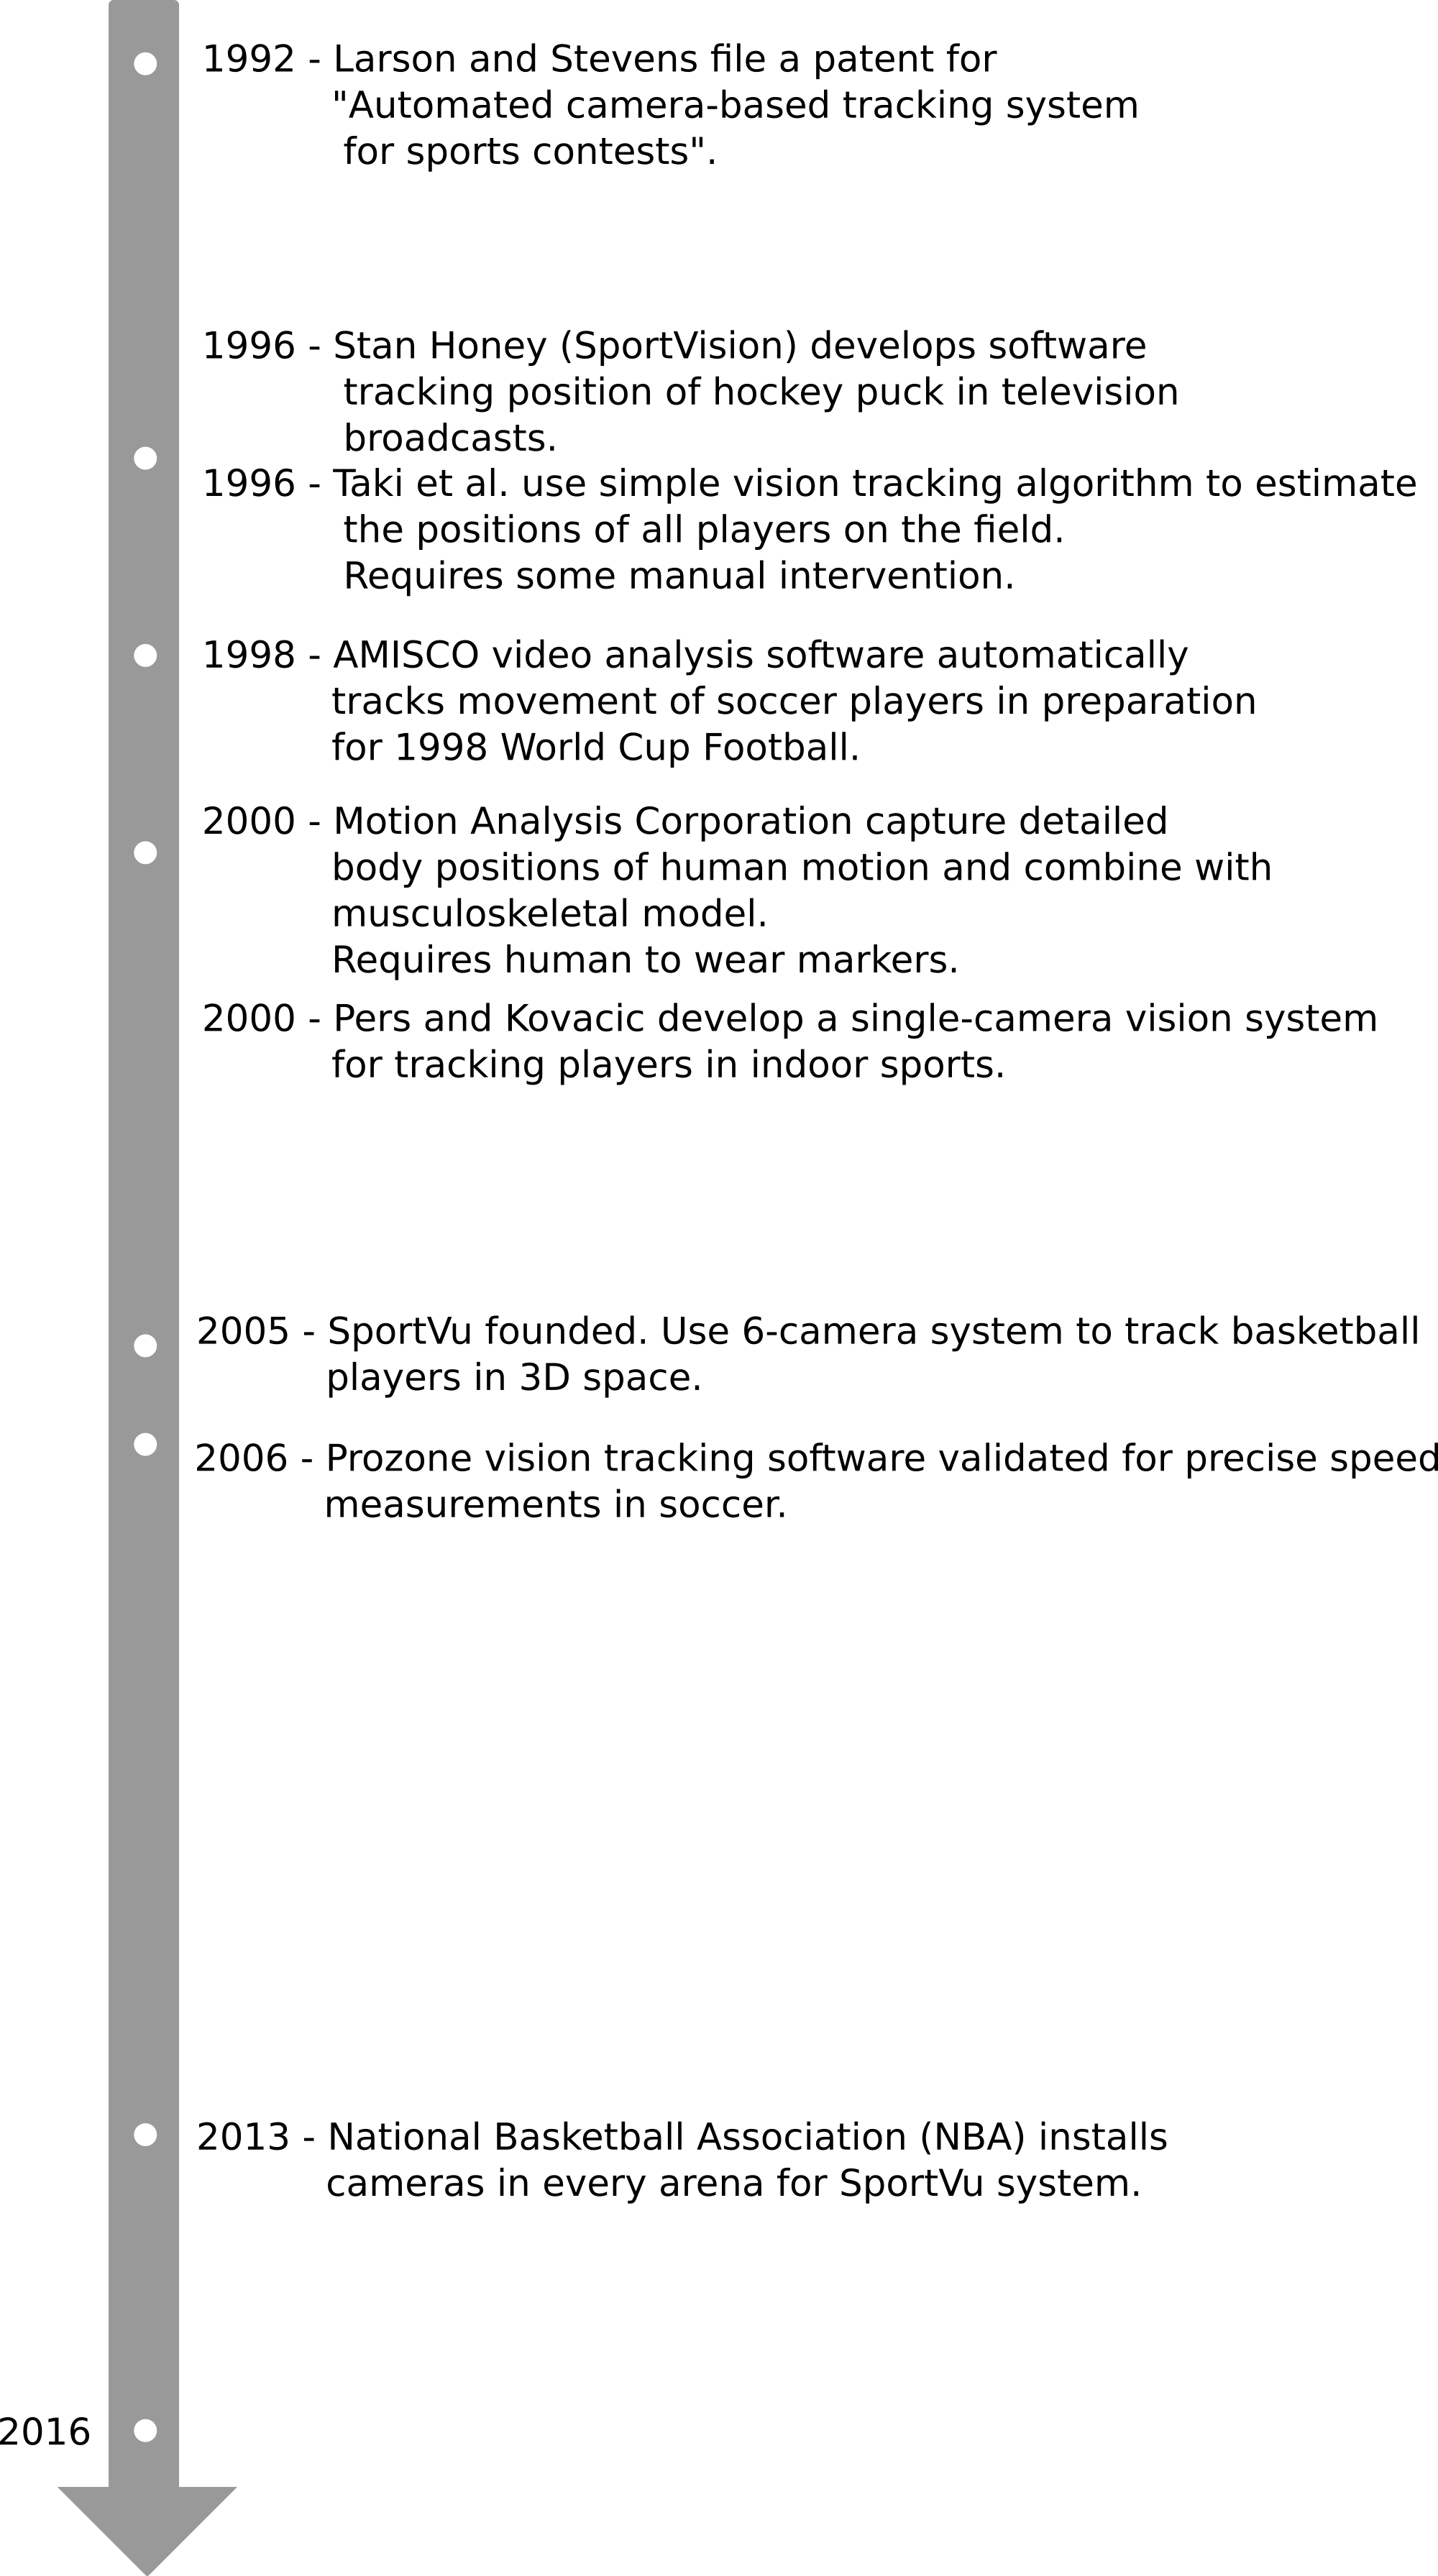
\includegraphics[width=0.8\linewidth]{figs/model/vision.png}
\caption{Timeline of Computer-Vision Tracking in Sport
\label{fig:vision}}
\end{figure}

Computer-vision systems provide a means of tracking all player positions
on the field. The key points of this section are presented visually as a
timeline in \figref{fig:vision}. For a review of the wide range of
sport tracking technologies available for use in Association
Football see Carling et al. \cite{carling_role_2008}.

In 1992, Noble G. Larson and Kent A. Stevens filed a patent for an
``Automated camera-based tracking system for sports contests''
\cite{Larson1994}. Their system uses an overhead camera and
simple background subtraction to detect the approximate location
of players. The patent admits the limitation that it will not work when
there is visual occlusion (i.e.~one player is hidden behind another in
the video image) of the players. Thus it will not work well if there are
``pileups'' as are common in AFL and other types of football. The system
does not have an automated means of identifying which player belongs to
which trace. Thus the patent suggests that a human operator manually use a
separate video feed to match the traces to the player identities. If
visual occlusion (e.g.~two players get too close to each other) causes
the tracker to become uncertain about which player is which, then a
human needs to resolve the ambiguity. An alternative suggestion was
combining it with ``telemetric data'' (i.e.~trigonometrically resolving the
locations of radio signals emitted from devices carried by the players)
to resolve the ambiguities. Despite being heavily cited by other sport
patents, the patent expired in 2003 due to failure to pay a maintenance
fee.

% \todo{check if president is the right term, and attempt to find archived version of dead link (might be in Zotero dump, but would need to host personal archive for examiners to use) (Yes: article calls him company's president)}
In 1996, Stan Honey (president of SportVision) developed software to
track the location of hockey pucks in order to highlight the puck on
television for easier viewing. SportVision went on to visualise the ``first
down'' line in American Football broadcasts.\footnote{Candice Shih,
  ``Drawing the line,'' 2002.
  \url{https://www.mv-voice.com/morgue/2002/2002_02_08.sportvision.html} Accessed:
  \dt{2018-12-13}}

In 1996, Taki et al. \cite{Taki1996} implemented a simple
vision tracking algorithm to estimate the positions of all players on
the field. Their system required a human to manually identify the
players in the first frame, and to manually re-identify the players
under certain situations such as if a player falls down. In the same
paper, Taki et al. introduced ``dominant regions'' as a means to analyse these data,
which will be discussed later in the Analysis of Spatio-Temporal Data section.

In 1998, VideoSports claimed to use its AMISCO video analysis software
to track the positions of players in preparation for the 1998 World Cup
Football.\footnote{Videosports, ``VIDEOSPORTS,'' 5~Apr~2001.
  \url{https://web.archive.org/web/20010405040646/http://www.videosports.fr/index2.html}
  Accessed: \dt{2016-03-17}} However, it is unclear how much manual user
intervention was required \cite{Baca2008}. VideoSports
competed closely with Prozone, a company founded for performance
analysis in sport, which also targeted products towards elite sport
teams \cite{Setterwall2003}.

In 2000, Delp (from Stanford University) and Loan (from Motion Analysis
Corporation) published a paper \cite{Delp2000}
describing a system that could combine a musculoskeletal model with
motion capture. The motion capture system used a technique known as
``stereophotogrammetry'' to create a three-dimensional image of human movements (such
as a volleyball spike) from multiple camera recordings with different
views. The musculoskeletal model was then used to infer the best
estimate of the underlying bone positions, which may not be obvious on
the surface. The vision system required physical `markers' to be placed
on the human to detect movements. Ordinarily, the vision system is used
in laboratory and studio environments rather than outdoor sport. The
motion analysis system has been used to study baseball pitches from
video recordings of the 1996 Olympics without markers; however, this
required humans to manually estimate the locations of body joints from
the video \cite{Escamilla2001}. Low cost
alternatives for tracking body positions in outdoor environments have
been suggested, such as covering the body with ultrasonic transmitters
and sensors to calculate the positions of body parts from the distances
reported by sensors (2007) \cite{Vlasic2007}.

In 2000, Pers and Kovacic described a system for tracking players using computer vision for indoor sport \cite{pers_computer_2000}. The system used multiple cameras for the purpose
of covering the entire field, but the algorithm was primarily concerned
with tracking using a single camera at a time. The authors found that a
combination of colour detection and ``template'' tracking (detecting
features such as edges or alternating colours) gave the best combination
of tracking ability and noise reduction. Manual intervention was
necessary when the system lost track of a player.

Later studies have described techniques for detecting players using blob segmentation (2001) \cite{barros_automatic_2001}, visualising ellipses of player movement (2005) \cite{Misuta2005}, %\todo{make it clearer what text each citation refers to} allowed tracking (looks even worse inside brakets)
tracking players in outdoor sport using a camcorder and the two-dimensional Direct Linear Transformation (DLT) procedure (2005)
\cite{Toki2005}, tracking \soccer{} games from TV
broadcasts (2006) \cite{Beetz2006}, tracking players
from a single moving camera using particle filters (2006)
\cite{Dearden2006}, and hybrids of manual and automatic
tracking (2007) \cite{Barros2007}.

In 2005, SportVU was founded by Michael ``Miky'' Tamir and Gal Oz who
both previously worked with Israeli military missile tracking
technology.\footnote{Z. McCann, ``Player tracking transforming NBA
  analytics,'' 19~May~2012.
  \url{http://espn.go.com/blog/playbook/tech/post/_/id/492/492}
  Accessed: \dt{2016-03-17}} \footnote{Israel21c, ``Israeli company turns
  televised sport into whole new ballgame,'' 2008.
  \url{http://www.israel21c.org/israeli-company-turns-televised-sport-into-whole-new-ballgame/}
  Accessed: \dt{2016-03-17}} However, Tamir's research on military tracking
technology is classified.\footnote{Business Wire, ``Idea sports
  entertainment group partners with israeli-based SporTVu, ltd., to
  launch patented revolutionary sports production technology,''
  10~Jan~2005.
  \url{http://www.businesswire.com/news/home/20050110005651/en/Idea-Sports-Entertainment-Group-Partners-Israeli-Based-SporTVu}
  Accessed: \dt{2016-03-17}} SportVU uses a system of six cameras to track
players\footnote{STATS, ``SportVU player tracking,'' 2016.
\url{http://www.stats.com/sportvu/sportvu-basketball-media/} Accessed:
\dt{2016-03-17}}, and was patented in 2006 \cite{oz_real-time_2009}.
Unlike previous systems that simply use multiple cameras to obtain more
complete coverage of the field, in SportVU, the different camera angles
are processed together to infer the position of players in three-dimensional space.
SportVU is primarily targeted at basketball. In 2013, the American
National Basketball Association (NBA) installed cameras in every arena
for the SportVU system\footnote{Associated Press, ``NBA arenas to have
  motion-tracking cameras,'' 6~Sep~2013.
  \url{http://espn.go.com/nba/story/_/id/9639224} Accessed: \dt{2016-03-17}},
allowing detailed information about every player to be captured and
published for coaches and sport fans.

% https://www.pixellot.tv/management-team/gal-oz-co-founder-and-vp-rd/
% Prior to Pixellot Gal  co-founded SportVu together with Dr. Miky Tamir (Pixellot’s co-Founder and Chariman

In 2006, Valter et al. conducted a study to validate the use of Prozone
to track players in \soccer{} under controlled conditions
\cite{Valter2006}. Players were asked to move at a variety
of speeds between precisely positioned ``timing gates'' at known
locations on the field. The study found that the system was able to
accurately measure speed when running in a straight line, as
demonstrated by a correlation coefficient of 0.999. However, the system
was not as reliable when a short 20\thinspace m sprint was combined with
a turn, which had a correlation coefficient of 0.950.

% Added based on feedback from associate supervisor that he didn't see the purpose in explaining the commercial history.
Development of sport monitoring devices and associated software is undertaken by large commercial companies that target their products towards elite clubs. Sport device manufacturers and software companies try to maintain commercial advantage by keeping the devices and software proprietary. Furthermore, elite clubs have an incentive not to share their current analysis techniques, as this allows them to maintain a competitive advantage over other clubs. As a result, descriptions of technology found in academic sport literature may lag behind the state of the art as implemented by commercial companies and only made available to those working in elite clubs. Therefore, it has been necessary to identify these companies and closely monitor any publications originating from them in order to gain glimpses of the state of the art.

Despite a long competitive history, many of the major companies that
offer player tracking for elite sport have been merged into STATS, LLC\footnote{STATS, ``Sports technology company,''
  2016. \url{http://www.stats.com/about/} Accessed: \dt{2016-03-17}}.
% https://www.vistaequitypartners.com/company/stats/
STATS acquired SportVU in 2008. VideoSports/AMISCO became SportsUniversal,
which merged with Prozone, then STATS acquired Prozone in 2015. STATS
and Catapult Sports (an Australian GPS tracking provider, which will be
discussed later) agreed to a partnership to integrate SportVU with GPS
tracking, for use in NBA.\footnote{T. Haberstroh, ``Now teaming up:
  Catapult and SportVU,'' 9~May~2014. Available:
  \url{http://espn.go.com/blog/truehoop/post/_/id/68143} Accessed: \dt{2016-03-17}}

In contrast to manually collected sport event data that record sparse
events usually relating to key interactions with the ball, video
tracking technology provides dense spatio-temporal data; i.e.~the
position of every player, at every moment in time. State-of-the-art
video tracking technology has matured to precisely track all players on
the field, as well as the location of the ball. Even with inexpensive %cheap ad-hoc
video recording equipment, vision tracking is possible, but suffers
from issues of visual occlusion when many players are in close
proximity.

%\pagebreak

\subsubsection{Development of Geopositioning Devices in
Sport}\label{development-of-geopositioning-devices-in-sport}

Geopositioning devices such as those utilising the Global Positioning
System (\gls{gps}) can be attached to players to track their movements during
the game. Often these devices contain a range of additional sensors such
as accelerometers, gyroscopes, magnetometers, and heart-rate monitors. One advantage of using geopositioning devices instead of
vision tracking is that this method doesn't suffer from visual occlusion
issues. The key points of this section are presented visually as a
timeline in \figref{fig:timeline}. For a review of the range of
commercial geopositioning devices used for tracking athletes see Maddison \& Ni Mhurchu \cite{Maddison2009}, Cummins et al. \cite{Cummins2013}, and Dellaserra et al. \cite{dellaserra_use_2014}.

\begin{figure}[htpb]
\centering
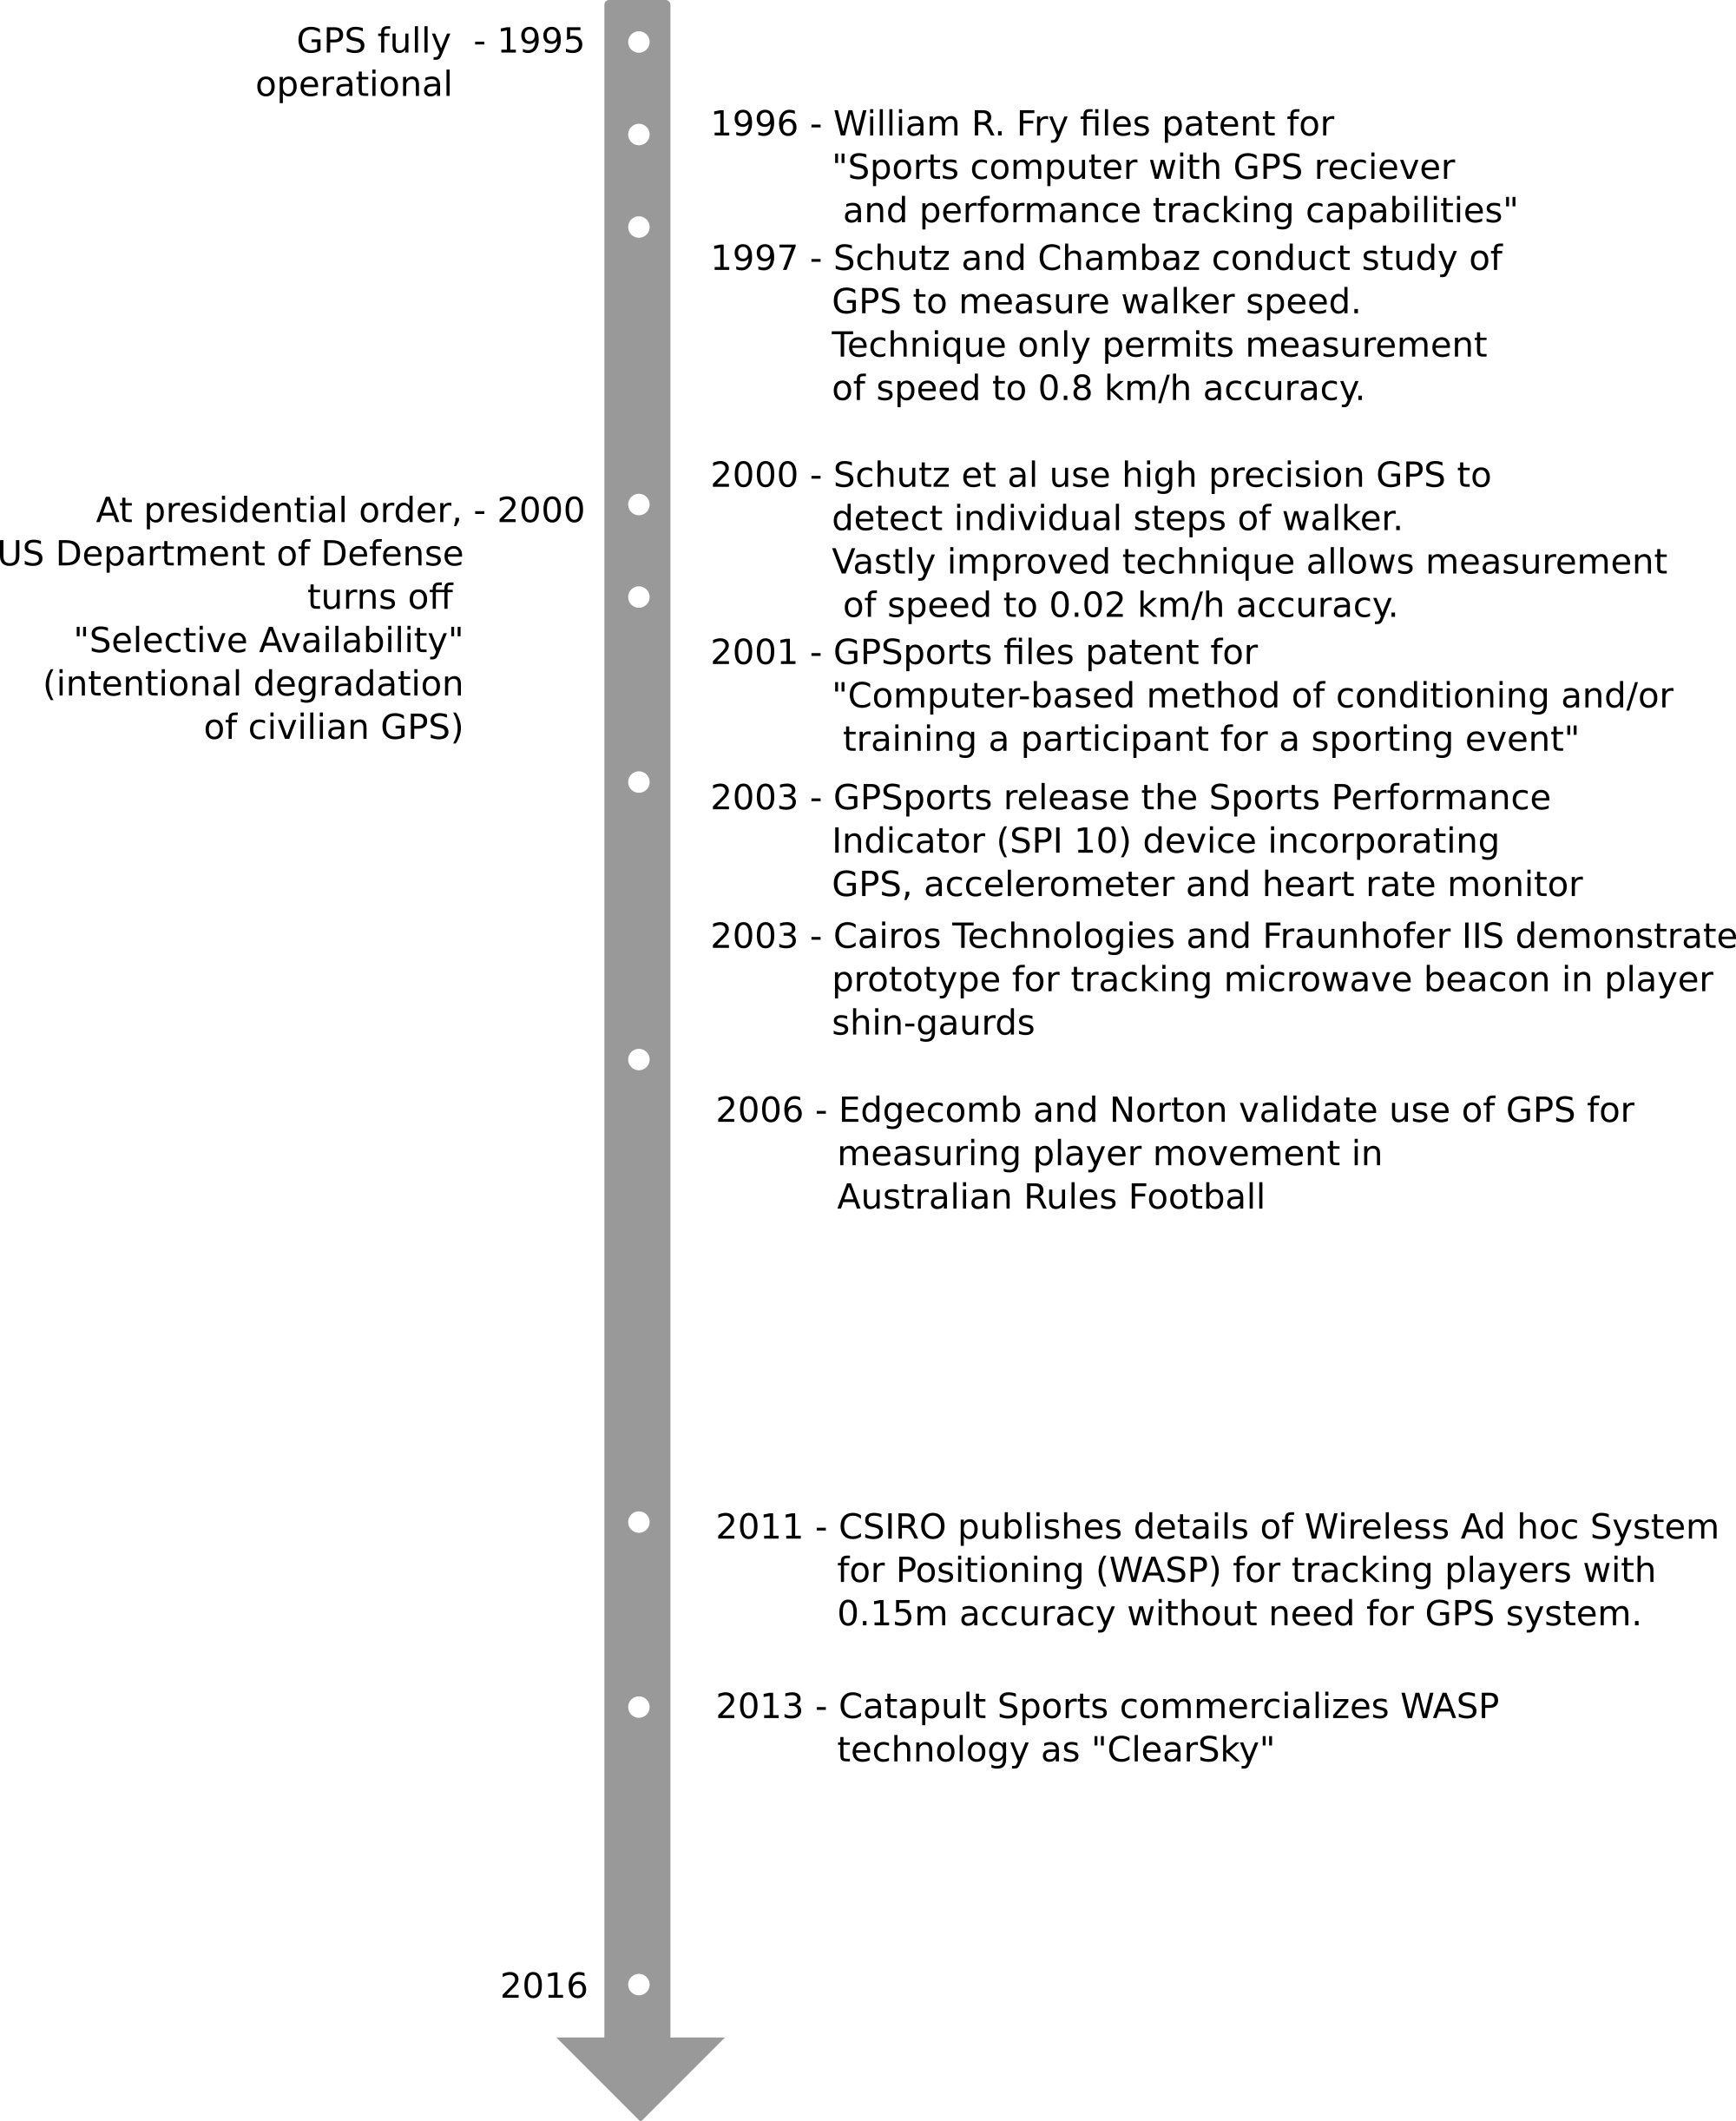
\includegraphics[width=\linewidth]{figs/model/timeline.png}
\caption{Timeline of Geopositioning Devices for \afl{} analysis\label{fig:timeline}}
\end{figure}

The first GPS satellite was launched in 1978 by the US Department of
Defense. The system has been fully operational since 1995.\footnote{Australian
  Maritime Safety Authority, ``GNSS navigation and horizontal datums,''
  May 2012.
  \url{https://www.amsa.gov.au/forms-and-publications/Fact-Sheets/GNSS_Fact.pdf}
  Accessed: \dt{2016-02-25}} The GPS system consists of 31
satellites\footnote{US Government, ``Space segment,'' 2016.
  \url{http://www.gps.gov/systems/gps/space/} Accessed: \dt{2016-02-25}} in
orbit about the Earth. Each satellite contains a high precision atomic
clock, and broadcasts its current time. GPS devices trilaterate % by means of trilateration https://en.wiktionary.org/wiki/trilaterate
their position on Earth based on the time delays between signal transmission
time reported by each satellite and the actual time the signal reaches
the GPS device (crudely, the distance to each satellite can be
calculated as the time-delay multiplied by speed of light; however, the
slowing and distortion of the signal as it passes through the atmosphere
complicates the situation). For accurate positioning, GPS devices
require visibility of at least four overhead satellites (to
%triangulate
solve for their position in four-dimensional space-time)\footnote{Trimble
  Navigation, ``GPS tutorial - getting perfect timing,'' 2016.
  \url{http://www.trimble.com/gps_tutorial/howgps-timing.aspx}.
  Accessed: \dt{2016-02-25}} \cite{Navstar1996}.

In 1996, William R. Fry filed a patent for a ``Sports computer with GPS
receiver and performance tracking capabilities''
\cite{fry_sports_2000}. In the original proposed form, the device
would attach to a bicycle, and log a range of sensors including GPS,
heart-rate, compass direction, and weather conditions. The patent has
since been assigned to Garmin International, Inc., which currently
manufactures ``wearable technology''\footnote{Garmin, ``Garmin,'' 2016.
  \url{http://www.garmin.com/en-US}. Accessed: \dt{2016-02-25}} for fitness
tracking.

Schutz and Chambaz \cite{schutz_short_1997} conducted what appears to be the
first \cite{Cummins2013} published study into utilising GPS
for sport. In the initial study Schutz considered the use of GPS to
measure walker speed. The GPS device used was a single frequency
consumer device, valued approximately 500 USD when the study was
conducted in 1997. Whilst the speed reported using GPS was correlated
with true walking speed, the error was as high as 0.8\thinspace km/h.
Schutz concluded that due to the large errors, GPS was ``insufficient
for research purposes''.

Selective Availability is a system where for ``national security
reasons'' the US Department of Defense programmed GPS satellites to
broadcast an intentionally inaccurate timing signal, with the deliberate
timing errors kept secret from the rest of the world. This degraded
civilian GPS, whilst allowing the Defense Department to correct the
errors and use GPS to its full precision. Finally in May 2000, at
presidential order, the US Department of Defense ended Selective
Availability\footnote{US Government, ``Selective availability,'' 2016.
  \url{http://www.gps.gov/systems/gps/modernization/sa/} Accessed:
  \dt{2016-03-01}}, thus removing artificial sources of errors. However, GPS
devices still suffer from errors beyond human control such as timing
delays due to the atmosphere.

In 2000, Schutz co-authored a paper using high-precision GPS to
investigate the individual steps of a walker
\cite{Terrier2000}. In contrast to Schutz's 1997
study, this study used differential GPS, in which a static reference
station placed within 100 meters of the receiver records signals from
the same satellites as the GPS tracker. As both devices experience the
same interferences, the differential GPS technique virtually eliminates
all sources of error, thus reducing positional accuracy from
%\todo{reword this to uncertainty / error radius} % reference calls it accuracy
10\thinspace m (typical GPS precision) % \nb{10 m or 3 m? Check what reference says} % reference says ``with an accuracy of about 10 m.''
% ``we achieve a theoretical precision better than 0.6 cm/s'' (speed)
% ``centimetric precision''
% ``From 100 m for a navigation solution measured with C-code only, we can reach a sub-centimeter pre-cision (Leick, 1995).''
to within 1\thinspace cm
(differential GPS). Furthermore, the GPS device was placed in
``differential carrier phase localization'' mode, which solves
mathematical equations for Doppler shift of GPS signals in order to
obtain better estimates of speed. Schutz (citing a 1995 surveying
textbook) claims that this should allow a theoretical precision of
0.02\thinspace km/h for measuring speed. Using this method, Schutz was able to detect the
small rise and fall of altitude occurring each human step. Schutz realised that
high precision GPS measurements were sufficient not just for typical
speed and position monitoring, but could be used to explore the detailed
characteristics of human movement.

GPSports (now owned by Catapult Sports) filed a 2001 patent for a device
designed for ``conditioning and/or training a participant for a sporting
event'' \cite{faccioni_information_2002}. The patent described a
device specifically targeted towards training elite players that contained a GPS and heart-rate monitor. %\todo{did it also mention an accelerometer?} (No. It assumes any accelerations are derived from GPS)
In 2003, GPSports manufactured
the SPI-10\footnote{GPSports, ``The sport performance indicator (SPI
  10),'' 19~Dec~2003.
  \url{https://web.archive.org/web/20031219215313fw_/http://www.gpsports.com/products.jsp}
  Accessed: \dt{2016-02-25}}, the first ``Integrated Technology'' to
incorporate GPS, an accelerometer, and a heart rate monitor
\cite{dellaserra_use_2014}.

In 2003, Cairos Technologies and Fraunhofer IIS demonstrated a prototype
for tracking players using a microwave beacon in player shin-guards. The
technology was reported to estimate positions with 5 to 8 cm accuracy
\cite{Beetz2005}. A 2016 evaluation
\cite{Seidl2016} using the RedFIR system
\cite{Grun2011} manufactured by Fraunhofer IIS found that
it could track the position of a fast moving football (soccer ball) with
a root-mean-squared error of 13\thinspace cm accuracy. The system was
originally intended for capturing Association Football matches, but
Association Football has resisted the use of technology in official
matches, and only allows goal-line technology (for determining whether a
goal has been scored).\footnote{FIFA, ``Blatter: Technology's time has
  come,'' 5~Jul~2012.
  \url{http://www.fifa.com/about-fifa/news/y=2012/m=7/news=blatter-technology-time-has-come-1660614.html}
  Accessed: \dt{2016-03-23}}

Edgecomb and Norton \cite{Edgecomb2006} validated the use
of GPS in 2006 for Australian Rules Football to measure the distance a
player moves. They found an error of approximately 7\%. An expertly
trained operator graphically tracking the player location on a computer
screen was able to achieve slightly better accuracy, but this was
obviously much more labour intensive compared to the GPS device.

In 2011, CSIRO published details of a Wireless Ad hoc System for
Positioning (WASP) \cite{Sathyan2011}. The WASP system allowed
tracking players with 0.15\thinspace m accuracy without the need for
GPS, thus allowing the system to be used indoors and in closed stadiums.
This was later commercialised by Catapult Sports as ``ClearSky''.

These technological improvements mean that coaches now have access to
high quality positioning data. However, anomalies and data gaps are
still to be expected, for example it is common for GPS signals to be
lost for a brief period of time. The additional sensors on tracking
devices open up a range of possibilities, for example accelerometers can
be used to measure the impact forces a player experiences when tackled
by the opposition \cite{Gastin2013, Gastin2014}. However, data collection companies %\nb{Champion Data?} (Actually claim was made by Catapult to argue they weren't replacing Champion Data)
claim that
qualitative data about the nature of interactions (e.g.~determining the
type of pass performed) still requires human observation.\footnote{Following a trial of ball tracking, Catapult Sports stated ``the reality is we can't decide whether that was a kick or a handball.'' A.
  Browne, ``AFL scraps smart-ball trial,'' 25~Feb~2013.
  \url{http://www.afl.com.au/news/2013-02-25/afl-scraps-smartball-trial}
  Accessed: \dt{2016-06-01}}

%\pagebreak

\subsubsection{Analysis of Spatio-Temporal Data}\label{analysis-of-spatio-temporal-data}

GPS tracking devices, vision tracking and other tracking techniques have
brought about a large volume of spatio-temporal data. Either geopositioning devices or vision tracking can be used to collect high-precision player trajectories over time at a high sampling frequency.
As such, the choice of technology is primarily to do with economic costs and regulations of the particular sport rather than one technology emerging as superior in all situations.
For example, GPS is typically better suited than vision tracking for large outdoor fields where it is difficult to mount overhead cameras or control for lighting conditions, but can suffer from problems with interference caused by the stadium structure. Unlike GPS devices, Radio Frequency based geopositioning devices can precisely pinpoint players without the need for satellite visibility, but require beacons to be pre-installed at the venue. Vision tracking is well suited to cases where regulations prohibit wearable tracking devices. Due to the ability of different data capture technologies to collect similar kinds of data, the analysis of the various tracking technologies will be considered together under the broader category of spatio-temporal data analysis.

A recent (2017) review of spatio-temporal data analysis techniques in sport is
given by Gudmundsson \& Horton \cite{Gudmundsson2016}. %In their review, %Gudmundsson and Horton
The review pays very little attention to the devices
themselves so as to maximise discussion of the analysis techniques used.
The review finds a diverse set of techniques, including dominant regions,
network analysis, and various visualisation techniques. However, there
is no consensus on which technique is the best, with little to no
validation of the practical value these techniques provide coaches or
players.

\begin{figure}[htbp]
\centering
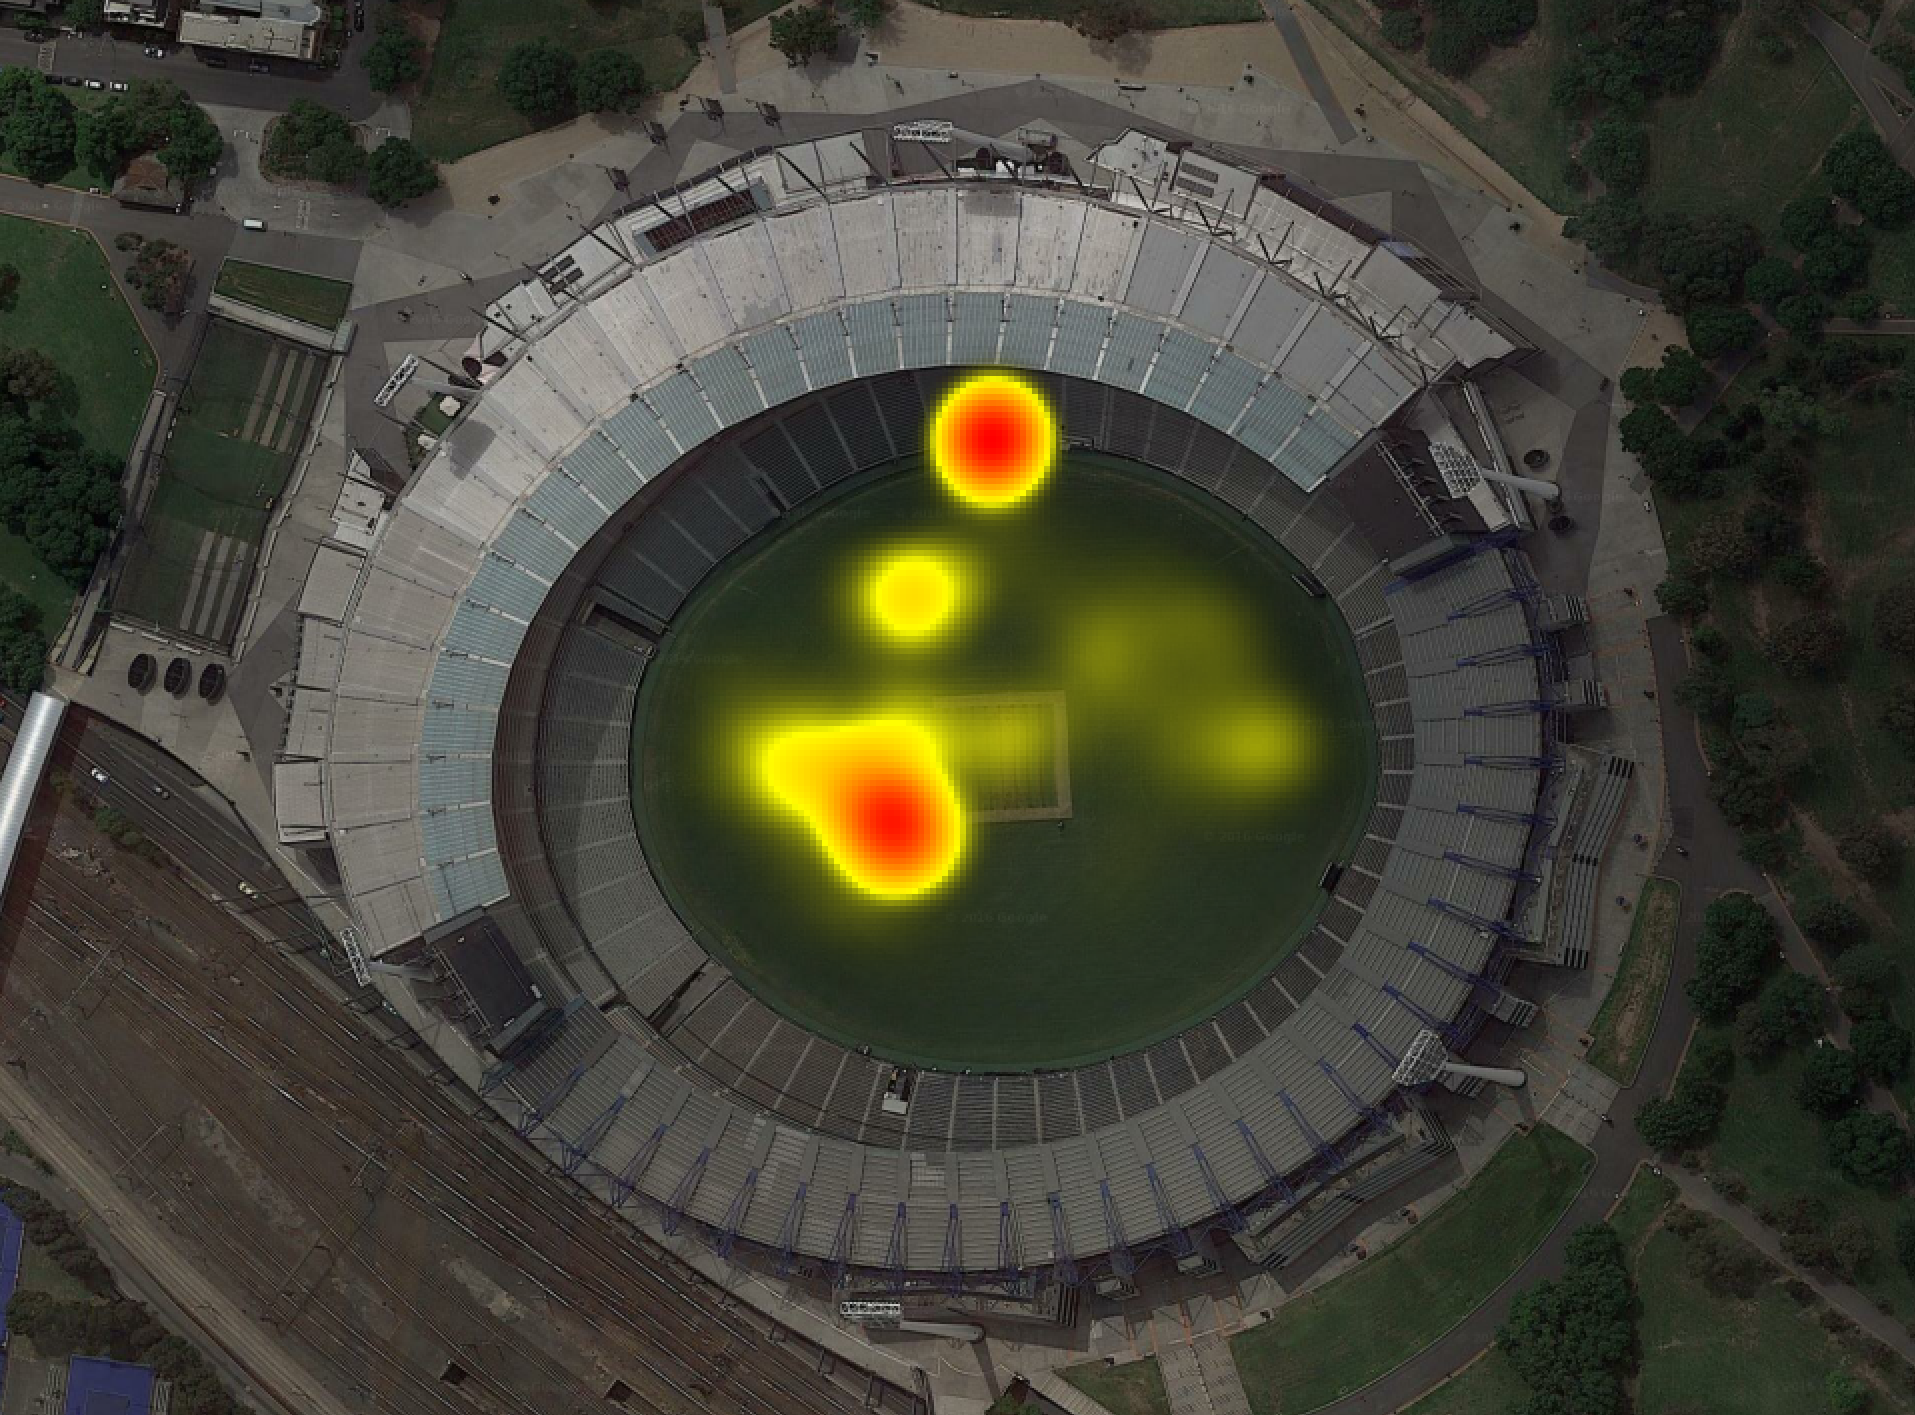
\includegraphics[width=0.9\linewidth]{figs/model/heatmap2.png}
% <NAME REMOVED>, 2015 AFL Grand Final
\caption{Heat-map showing positions where a particular player (name removed for privacy reasons) spent the most
time during an AFL match.
% in the 2015 AFL Grand Final.
The heat near the north edge of the
stadium is the interchange area. Background imagery \copyright{}2019 Google. \label{fig:heatmap}}
\end{figure}

One popular tool for analysing spatio-temporal data is to create a
heat-map \cite{Jackson2016}. Spatial data are aggregated by location. A exponential
time-decay factor can be introduced to discard old data, so that the
heat-map only shows recent activity. The heat-map can reveal insights
into which areas of the field the ball moves in, which areas of the
field the players are covering, as well as any gaps that the player(s)
might be missing. An example heat-map to visualise the
positions of an AFL player is presented in \figref{fig:heatmap}.

Inspired by the concept of ``equity'' in backgammon, defined as ``the value of a position to one of the players''\footnote{Keith, ``Backgammon Glossary'' \url{http://www.bkgm.com/glossary.html\#equity} Accessed: \dt{2018-12-13}}, O'Shaughnessy applied this concept to AFL
\cite{oshaughnessy_possession_2006} to produce plots of the expected value of ball possession over the surface of an AFL field. O'Shaughnessy showed how this in turn can be used to produce an estimation of the expected game outcome conditioned upon the current score, ball position, and the team with ball possession. O'Shaughnessy's plots show that the value of possession increases steeply near the 50 metre from goal line, as this is the distance that most players can kick a goal from. The value a player brings to the team can be assessed by how their actions increase or reduce the expected team score.

% \footnote{Karl Jackson is an employee of Champion Data (the official AFL statistics provider), thus had access to data relating to all teams}
Karl Jackson built upon this concept to design the official AFL player ranking system. The concept is outlined in one of his early papers \cite{Jackson2008}, and the full details of the completed system are in his thesis \cite{Jackson2016}. Players are rewarded points for the value their actions bring to the team. For example, a player that manages to successfully traverse the ball through a difficult region of the field where it would usually be lost to the opposing team will be rewarded highly. In contrast, if the player handballs the ball to a player nearby
without incurring any risk or delivering any value, then they will not be delivered many equity points for this manoeuvre.

In a recent paper presented at \textit{MathSport 2018}, Spencer et al. \cite{Spencer2018} demonstrate that equity can also be used to evaluate player decision making by comparing the expected outcome (defined in terms of the change to equity) of a passing decision made by a player to the expected outcome of the best alternative option available. This has only been possible recently, due to the need for: position tracking data to determine the locations of players open for passing to; tracking data for the opposition team to determine players that might try to contest the possession; and a model of reachable regions to determine how far players will be able to move in time to catch the ball taking into account their current direction and speed. The authors of the paper noted a weak \textit{negative} correlation between decision making and score margin (i.e. teams that made better decisions according to the model performed slightly worse), which highlights the early stages of this research and need for further work to refine the decision evaluation model. Players passed shorter distances than the theoretically better options available further away. The authors of the paper speculated that this may be due to obstruction of visibility. In \secref{sec:shapepaper}, this thesis will offer an alternative explanation: moving the ball forward quickly does not leave time for the team to restructure itself around the ball, and is strongly associated with team spread. Thus players may be factoring in other considerations not present in the theoretical model, such as the disruption to the desired team shape.

%expected points model
However, the current expected value model used to calculate equity rankings in AFL is solely dependant on the manually annotated position of the ball\footnote{Ball position is manually pinpointed by Champion Data employees who monitor each AFL game.} and possession state. While Spencer et al. \cite{Spencer2018} used player position tracking data to examine decision making options available, the underlying equity model utilised to evaluate those options was solely conditioned on ball position and possession and thus does not consider the implications of a pass that leaves the team in an undesirable formation. Ideally, the modelled state of a game should go beyond just ball position and possession to also consider the position of players on the field. Evaluation of decisions should look beyond the immediate passing opportunity to consider whether this will leave the team in a good position for subsequent passing opportunities. An example of this is the work on Expected Possession Value (EPV) in basketball \cite{Cervone2014} which provides a mathematical framework for computing the expected points arising from a possession considering all known information about the ball and position of players on both teams at a given time (similar to a stock ticker). Computing this efficiently requires modelling the game at different spatio-temporal granularities \cite{Cervone2016}.

In a similar vein to O'Shaughnessy's contour plots of expected value, St\"ockl and Morgan introduced the ``isopar'' visualisation (a play on the name ``isobar'' used in meteorology)
\cite{Stockl2011}. The isopar visualisation displays contours
representing the expected score from any position in a game of golf. In
2013, they adapted this visualisation for the purposes of analysing
scoring positions in hockey \cite{stockl_visualization_2013}. For
hockey analysis, they used association rules mining to infer the value
of positions. The visualisation revealed asymmetry of goal-shooting
positions in hockey, due to the left/right handedness of the players.

%Of interest in many studies, is the question of how to suitably
%discretize the field into cells. % (not sure how this would work - the dominant regions are dynamic)
In 1996, Taki et al. \cite{Taki1996} suggested the concept of ``dominant
regions'', which is inspired by Voronoi regions and Delaunay
triangulation popular in geometry and computer graphics. The dominant
regions are defined for each player as the set of points that they can
reach before any other player. In 2014, Gudmundsson et al. \cite{Gudmundsson2014} integrated
dominant regions into a software tool for providing coaches with
strategic insights.

In 2002 McGarry et al. described sport as a dynamical system
\cite{McGarry2002}. Plotting the distance of squash players from centre-court vs time, they observed a sinusoidal waveform representing the to-and-fro of each player as they move out to hit the ball then return to a more neutral position. Superimposing the plots of both players, they observed that there
appeared to be an invisible coupling between the two players, and
measured the phase offset between the two position-vs-time plots.
Through closer inspection of the superimposed plot, they explained how
the characteristics of the plot could be explained using a dynamical system
model consisting of periodic oscillators, lead-lag relationships, and
damping.

Of particular interest, is the introduction of ``perturbations'' to the
dynamical model. In sport notational analysis, perturbations are defined
as events that disrupt the control characteristics of the dynamical
system, causing it to fundamentally alter it's nature. McGarry et al. \cite{McGarry2002}
suggested that players deliberately create perturbations to upset the
status-quo of the rally, allowing them to break the defence of their
opposition. The role of these instabilities in determining rally
outcomes explains the difficulty that McGarry et al. initially had
establishing consistent behaviour profiles for players in their earlier
1996 \cite{McGarry1996} study.

After Disney acquired the ESPN sports entertainment network, Disney
focused research effort into the automated analysis of sport games. In
2014, Bialkowski et al. (from Disney Research and Queensland University)
used clustering as a means of automatically identifying player roles
from position traces \cite{Bialkowski2014}.

Numerous machine learning techniques have been proposed to exploit the
spatio-temporal data for predicting various attributes of the team
\cite{Hughes2004}. Grunz et al. \cite{Grunz2009} proposed that self-organising maps (a specialised form of neural
networks) may be used to model player creativity.

RoboCup is a competition in which physical or simulated autonomous
robots compete in an \soccer{} inspired competition. The competition has inspired
research into formalising strategy. Of particular interest is ISAAC (ISI
Soccer Automated Assistant Coach) \cite{Nair2004}, an automated coaching assistant that
analyses logs of the game using decision tree induction \cite{Quinlan1993} to learn rules and suggest strategy modifications to
improve performance. % The performance patterns of each team are data-mined as formal ``action-probabilistic'' rules.
Beetz et al. \cite{Beetz2005} suggested that a similar approach could be
applied to player traces of real \soccer{} games, and suggested that the
the rules could build upon each other to express high-level strategies.

% Ghosting by Disney research and STATS
In 2017, Le et al. \cite{LeHoang2017} were able to simulate expected team positioning behaviour using team spatial data in \soccer{}. They trained an LSTM model (a type of recurrent neural network) to predict the expected position of defending players given the position of the attacking team. The expected positions can be overlaid (as player ``ghosts'') on a visualisation of the actual player positions to determine when a player is out of formation. Preparing data to feed to the LSTM model required construction of a computational pipeline with multiple sub-steps that feed into each other, such as data cleansing, determination of consistent indexes for players based upon their role, feature extraction, neural network training, inference, and visualisation. In 2018, Seidl et al. \cite{Seidl2018} applied this to the context of basketball. They demonstrate a system whereby the coach digitally sketches their planed play on a tablet computer, and the system in turn automatically visualises how the opposition team is likely to position themselves in response.

%\pagebreak

\subsection{Gaps}\label{sec:gaps}

This section provides a list of gaps identified through the review. The extent to which this thesis will address each identified gap is outlined in \secref{sec:gap-rq-mapping}.

% \nb{The gaps below were observed during the initial literature review, but do not necessarily reflect the final direction of this thesis. While the literature focuses on presenting novel analysis techniques, the focus of this thesis is on understanding the data processing components required to build a platform to permit meaningful and reproducible sport analysis (which while important, is often overlooked or left undocumented in the literature).}

\textbf{Gap 1:} There has been a proliferation of sport metrics and analysis approaches. While it is trivial to compare accuracy of predictive models for betting purposes, these do not necessarily deliver insight to players and coaches. As Domingos \cite{Domingos2012} explains in his informal review of Machine Learning:

\begin{quote}
``learners are typically compared on measures of accuracy and
computational cost. But human effort saved and \textbf{insight gained},
although harder to measure, are often more important.'' \cite{Domingos2012}
\end{quote}

Which sport analysis approaches provide sport practitioners with the deepest insights, and how can insight be measured?

% Sports scientists have performed intervention studies to empirically
% compare the efficacy of competing feedback metrics for enhancing closed
% skills (predictable environment), such as target shooting (e.g.~shooting
% error presented to the athlete using an audio signal). However, this is
% much more difficult for decision-based open skills (unpredictable
% environment) in team sport, as the long-term results of a decision are
% not immediately observable. Which approaches provide players and coaches with the deepest insights, and how can we measure insight?
%  Which metrics are good heuristics for
% predicting how a decision impacts upon the final score? Which metrics
% provide players and coaches with the deepest insights, and how can we
% measure insight? Which metrics suffer from perverse incentives? How many
% games must be studied before a metric can reliably evaluate a player?
% Can we design a single metric that possess all these qualities
% (predictive, insightful, no perverse incentives, reliable), or must we
% trade-off some qualities for others?

% As Gregor explains in \emph{The Nature of Theory in Information Systems}
% \cite{gregor_nature_2006}, a theory for \emph{design and action}
% depends upon a \emph{theory for predicting} (predictive models) as well
% as a \emph{theory for explaining} (analytical models).

\textbf{Gap 2:} Researchers have used a range of different
Markov models for sport, with varying numbers of states
defined by various attributes. However, Markov models used in AFL currently only focus on the position of the player with the ball and do not incorporate the position of other team-mates.

How can the state explosion that occurs from the combination of all possible team formations be handled? What are the full set of attributes needed to describe the state of an AFL game (player positions, player velocities, player fatigue, ball
position, time remaining, score margin, communication received, etc.), and which of these attributes can be discarded or summarised while still providing a
reasonable approximation?

%  How should we select the states to allow
% the best prediction without the problem becoming computationally intractable?

\textbf{Gap 3:} Technology has advanced to the point that there
now exists a large volume of high-precision spatio-temporal data. Whilst
theoretically valuable, it remains an open problem as to how this data can
be practically utilised for tangible gains:
% Similar sentiments are echoed
% by many scholars:

\begin{itemize}
\item
  ``sensed positional data contains an \textbf{enormous amount of
  information} that must be \textbf{correctly abstracted} to give
  coaches optimal support for controlling the competition''
  \cite{Beetz2005}
\item
  ``Several companies offer the ability to track the position of the
  players and the ball with high accuracy and high resolution. They also
  offer software that include basic analysis tools, for example basic
  statistics about distance run and number of passes. It is, however, a
  \textbf{non-trivial task to perform more advanced analysis}.''
  \cite{Gudmundsson2014}
\item
  ``there is a vast amount of literature on tracking objects from video
  and hardly any research on \textbf{analysing the obtained movement
  data}.'' \cite{Gudmundsson2014}
\end{itemize}

What will be the \emph{killer app} (seminal software that gives value to a platform) for spatio-temporal sport analysis?
% that is powered by this spatio-temporal data?

\pagebreak{}

\section{Chapter Summary}\label{sec:gap-rq-mapping}

The review identified 3 key gaps: 1) the lack of an agreed upon definition of ``insight'' in the sport literature, 2) that existing models of AFL focus on the ball rather than the team, and 3) there is no open platform for spatio-temporal team sport analysis. This section explains how the thesis research questions (defined in \secref{sec:questions}) contribute toward filling these gaps (detailed in \secref{sec:gaps}). The mapping is shown in \figref{fig:map-gaps-to-rq}.

\begin{figure}[htbp]
\centering
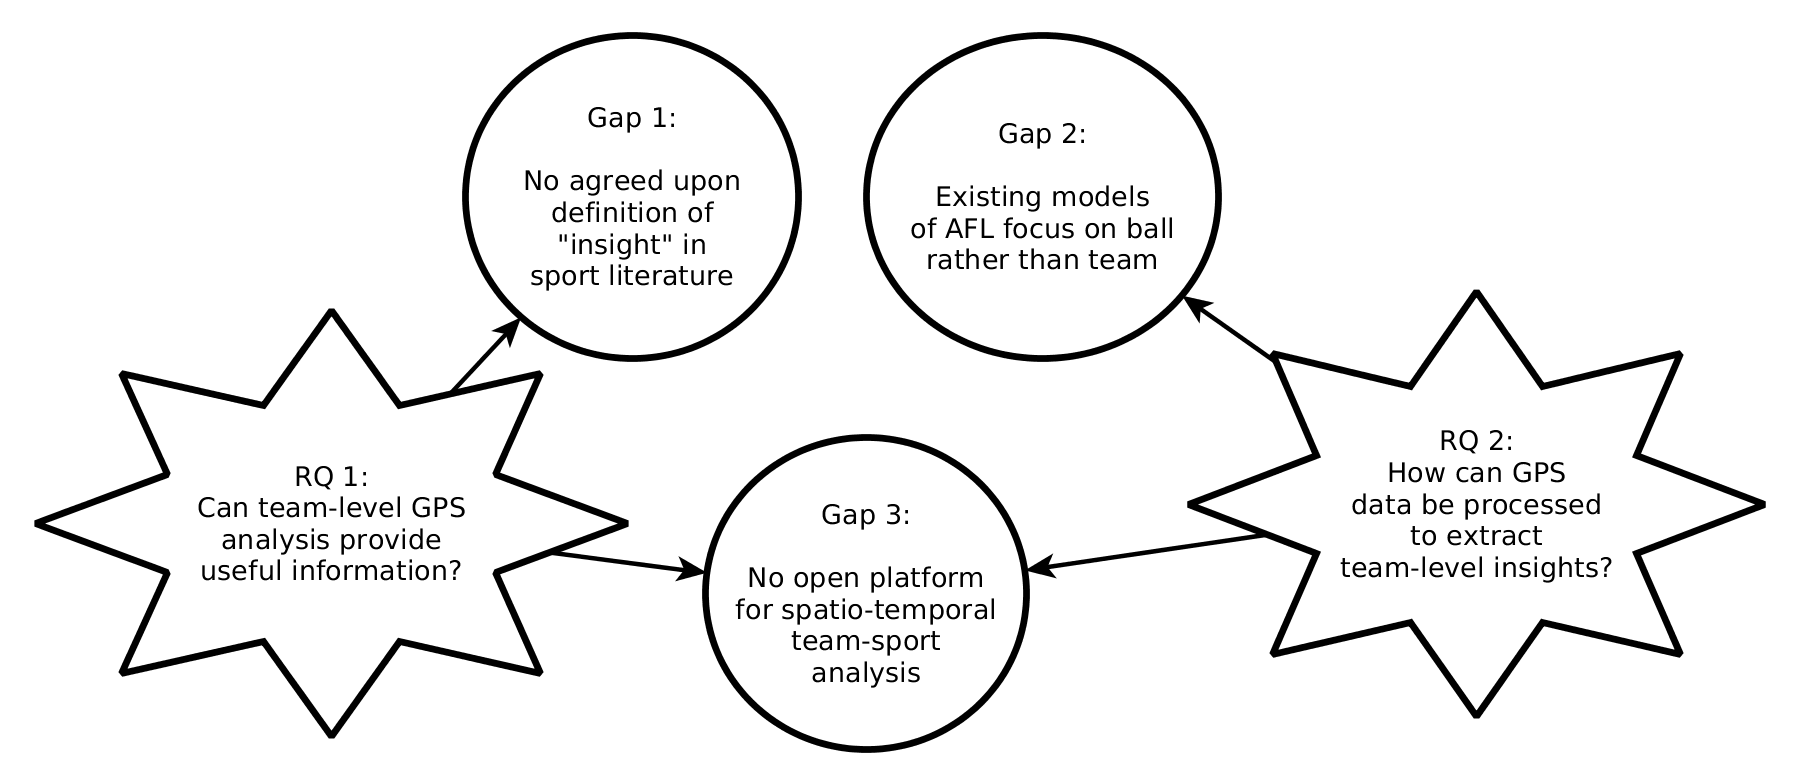
\includegraphics[width=1.0\linewidth]{map-gaps-to-rq.png}
\caption{Mapping of Research Questions to Gaps}
\label{fig:map-gaps-to-rq}
\end{figure}

\subsection*{Addressing Gap 1}

Research Question 1---\textit{can team-level GPS analysis provide useful information to sport researchers and practitioners beyond what they already know from manual observation, video analysis, traditional statistics, and (individual) player GPS monitoring?}---contributes toward filling Gap 1 through providing an example of an approach that is useful to sport practitioners, i.e. that offers insights that can help understand the game (in contrast to betting models that solely attempt to predict game outcomes). In particular, \chref{ch:modelling} provides theoretical modelling of the problem in terms of player feedback (\secref{sec:feedback-model}) and information theory (\secref{sec:info-theory-perspective}) in order to reason about which types of solutions are most likely to offer meaningful insights.

\subsection*{Addressing Gap 2}

Research Question 2---\textit{how can GPS player tracking data be processed to extract meaningful team-level insights without compromising individual privacy?}---contributes to filling Gap 2 through considering the team formation, and not just the player with the ball. \secref{sec:model-of-afl} provides a full list of all identified state variables involved; however, the thesis focuses on the team formation, in particular the team spread. \chref{ch:de-identification} deals with the challenge of representing the team formation without revealing individuals.

% This is demonstrated through an investigation of how AFL team formations spread/contract in defence/offence (\secref{sec:shapepaper}).

\subsection*{Addressing Gap 3}

Gap 3 pointed towards the quest to develop a \textit{killer app} that will offer sport performance analysts with unprecedented strategic insights into the game through uncovering patterns previously hiding in the wealth of data now collected on players. While the work in this thesis is demonstrated through a minor contribution toward better understanding how AFL team formations spread/contract in defence/offence (\secref{sec:shapepaper}), this is not the main goal of the thesis.

Rather, by addressing Research Question 1 and Research Question 2, the aim of this thesis is to create a platform that facilitates further spatio-temporal analysis of team sport. This requires consideration of the computational pipeline framework (\chref{ch:prov}), de-identification operations (\chref{ch:de-identification}), and spatial normalisation operations (\chref{ch:spat-trans}) involved. While the importance of these topics is well established in the software engineering literature, these details are often overlooked entirely in the sport science literature. Each stage is designed with consideration of Human--Computer Interaction (HCI) concerns, such as permitting sport performance analysts to trace results back to relevant video footage, safely de-identify data when sharing them with researchers, and manage reference frames without the need to master GIS.
